\chapter{Methodology}

For this assignment we decided to explore different methods to create sound with the DAC for the EFM32GG in order to have a solid basis of comparison for both energy efficiency and overall sound-quality. The two different approaches we settled on were sample playback using samples synthesized before runtime. The other approach was using an on board synthesizer creating square waves on the go. Before detailing the different approaches we will describe the necessary setup for both approaches.

\section{Simple Sound Generator}
In order to get an introduction to programming the DAC we created a program intended to play a static sound. This would be an easy introduction to C programming, and would give us a good performance baseline with regards energy expenditure.

\subsection{GPIO and Clock Setup} 
The first step was porting the assembly code we had previosuly written to control LEDs and clocks over to C. Having set up the LEDs and buttons would also make it easier to debug the code by writing values to the LEDs to discern the current program state. Rather than starting with a simple polling loop we felt confident enough to go straight to interrupts for the LEDs and buttons, letting the program idle in a loop between interrupts. In addition to GPIO we also activated the timer module TIMER1 so we could produce steady interrupts in order to generate sound.

%%Some code for the handlers maybe%%

\subsection{DAC Setup}
In order to generate a tone setting up the DAC was necessary. For the first program the configurations suggested by the compendium were used

%%Some code for setting up DAC%%

Having set up the DAC writing a value represented by 12 bits would change the voltage of the DAC. In order to generate sound we needed to oscillate the DAC which we did with the timer interrupt we had set up. Using a simple conditional statement we oscillated the DAC voltage between 0 and 1000. Our first attempt was outside of the audible frequency range, but by adjusting the timer we could reduce the amount of interrupts to control the frequency.

\section{Efficient Interrupts}
After setting up everything we needed to generate a simple tone we decided on some preliminary optimizations to our program. Rather than using the TIMER1 module we used the LETIMER with a max speed of 32678 hz, more than ample for our needs. Going away from using the regular TIMER also allowed us to go as deep as energy mode 2, turning off the HF clock between samples.

\subsection{LETIMER Setup}
In order to use the LETIMER, we configured the CMU through the following steps:
\begin{itemize}
  \item Starting the Low Frequency Oscillator LFXO by writing 1 to the LFXO bit in CMU\_OSCENCMD.
  \item Setting LFXO as a clock source for the LFACLK clock by writing 0 to the LFA bits in CMU\_LFCLKSEL.
  \item Enabling the LFACLK clock for the LETIMER by setting the LETIMER0 bit in CMU\_LFACLKEN0.
  \item Enabling the clock for the low energy peripheral interface by setting the LE bit in CMU\_HFCORECLKEN0.
\end{itemize}

% TODO: Explain how we needed to configure the registers
\subsection{Clock Accuracy}
We first used settled on the LFRCO clock as a timer, hpwever we experienced weird sound artifacts. This was most likely due inaccuracy in the LFRCO itself. It seems that we had no guarantee that the frequency was excactly 32.768 Hz, and as a result we changed to LFXO, which gave a stable sound.

\section{On Board Synthesizer}
Limited memory is a consern on for the EFM32 board and as a result we wanted to create a synthesizer. A song is stored in memory as integer arrays. The integer array contains information to create different tones. Two integer arrays produces a song with two channels.

\subsection{Song Representation}
Our first thougt was to save all the samples of a song. A song is usually sampled at 44100 Hz and each sample is need 2 bytes. One second of a normal song takes about 86 KB. However, the EFM32 board has a limited amount of memory. We could have managed to represent a few seconds of high quality sound with optimizations. In our solution we chose to represent a song as an array of 16 bit int values. These arrays is generated by a python script and placed in the source code. Inside these 16 bits we store information about pitch, octave, amplitude and duration. In table \ref{tab:bitFields} the bit partitions are described.

\begin{table}[H]
	\begin{center}
	\begin{tabular}{ |c|c|c|c| }
	  \hline
	  Duration & Amplitude & Octave & Pitch \\
	  \hline
	  5 & 3 & 4 & 4 \\
	  \hline

	\end{tabular}
	\caption{Bit partitioning}
	\label{tab:bitFields}
	\end{center}
\end{table}

Each pitch value is represented by a value from 0 to 11. The Octave can take the values 0-10. Note A with octave 0 is lowest possible at 27.5 Hz, and note A with octave 10 the highest at 28160 Hz. DAC's lowest values is to low hear, beacuse of this we calculated the amplitude with the equation \ref{eq:amplitudCalculation}. In addition we only had 3 bit to store the amplitude values, and as a result we calculated it exponentially. Duration takes values between 0-32. In our program we define the duration of the shortest note. The duration value is multiplied with the defined duration value and returns each notes duration given in milliseconds. By changing the defined duration value we can increase or decrease the song's speed.

\begin{equation}
  x = 2^{amplitude + 5}
  \label{eq:amplitudCalculation}
\end{equation}

\subsection{Song Playback}
To play a song the synthesizer wakes up 32768 times every second. Each tone is played with square waves. After calculating each tone's frequency the synthesizer turns the DAC on and off, to match the tone frequency. This method has limitations when it comes to reproducing sounds, but this metod is very space efficient.

\section{Sample Based Music Player}
An issue with the synth is that in order to generate more advanced waveforms a program must utilize expensive trigonometric calculations to express them. Although the EFM32GG does have the capability to generate a sine wave on the DAC, in order to play actual music a more advance approach is required. To achieve this we decided to do the expensive calculations on a personal computer, using a synthesizer to sample a sine wave and output an array that could be compiled. Although the limited DAC sound quality made it possible to use a fairly low sample rate with no discernable quality difference we settled on using the maximum sample rate the LFXO clock could grant us, 32768 samples per second. 

\subsection{Song Representation}
In order to play back sound at a given sample S with B bits accuracy the required data is S*B per second. for 12 bits accuracy at a 32768 samples per second that equates 48kB for a second of music, unfeasible for the 128kB of SRAM the EFM32GG has. Additionally, in order to simplify access to sample the 12 bit values would be loaded into 2 bytes, effectively making each 12 bit sample take 16 bits of storage. In order to save space we therefore decided to create samples of the frequencies we needed into short segments that could be repeated as long as we wanted the sound to play. To implement this idea we created an array with 100 sample pointers as a lookup table for notes, where every note was assigned its own number, initializing only the pointers that pointed to a note that would be played. A song could then be encoded as an array of instructions to access various notes and repeat the sample for a set duration.


\begin{figure}[ht]
  \centering
  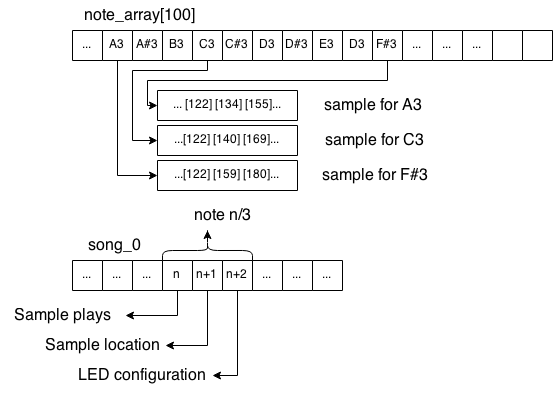
\includegraphics[width=\textwidth]{images/sample_array_layout.png}
  \caption{A map of the memory layout for the sample based approach}\label{fig:array_layout}
\end{figure}

\begin{minipage}{\textwidth}
\begin{lstlisting}
typedef struct Player
{
	uint16_t song;			// Number of current song
	uint16_t song_len;		// Total notes for current song
	uint16_t notes_played;	// Keeps track of notes
	uint16_t sample_total;	// Times current sample should play	
	uint16_t sample;		// Times current sample has played
	uint16_t sample_i;		// Position in current sample 
	uint16_t note_len;		// Length of current sample
	uint16_t* note;			// Location of current sample
	uint16_t LED;			// Current LED configuration
} Player;
\end{lstlisting}
\end{minipage}

\subsection{Song Playback}
In order to play a song we bundled the necessary attributes to keep track of what notes to play and their tempo together in a Play struct. To initialize a song play\_init() is called with the song to be played as the argument. This sets up a playback. After initializing calling the play() function will output the next sample to the DAC.
The play() function keeps track on the current position of a playback, reading from an array of triplets to load the next note whenever the current one has been finished. \\

\begin{minipage}{\textwidth}
\begin{lstlisting}
void play(void){
	// Load the next sample
	if(player.sample_i < player.note_len-1){			
		player.sample_i++;								
	}
	else{								
		player.sample_i = 0;
		if(player.sample < player.sample_total){
   			player.sample++;				
		}
		else{							
			player.sample = 0;
			if(player.notes_played < player.song_len){
				next_note();
				(*GPIO_PA_DOUT) =  player.note_len << 8 ;		
			}			 
			else{
			  disableLETIMER();
			  disableDAC();
			  //__asm("wfi");
			}
		}
	}
	// Write the sample to the DAC
	*DAC0_CH0DATA = player.note[player.sample_i];
	*DAC0_CH1DATA = player.note[player.sample_i];
}
\end{lstlisting}
\end{minipage}



\section{Testing}
In order to test the functionality of our program we relied on visual and aural feedback rather than software approaches such as GDB. By using the LEDs we could write values directly to the LEDs, and with the earphones we could hear whether the sound was playing correctly or not. In order to measure energy consumption we used the onboard LCD screen for quick estimates. For more quality measurements we used eAProfiler on a PC to read energy consumption on the board via the USB connection. In order to get quality measurements we performed them all in succsession on a board that had been in use for several hours to minimize measurement variance. 

\section{Optimization}

% stuff
As a considerable energy reduction was achieved by entering by entering energy mode EM1 after writing samples to the DAC, it was natural to think that entering EM2 would lower the energy reduction even further. One issue that occurred while implementing this functionality, is that the TIMER used to generate interrupts for the microcontroller is only available in energy modes EM0 and EM1. Thus if the microcontroller is to enter EM2 or lower energy modes, a different source of interupts is needed. The EFM32GG implements this functionality with the LETIMER module introduced in section \ref{sec:letimer}.

% TODO: Put this section somewhere appropriate
% TODO: Write about how using interrupts to sleep between each sample written to the DAC saves energy
\subsection{Sleeping Between Interrupts}
During music playback the board recieves 32.768 interrupts each second. In the time between interrupts we placed the board in sleep mode. We tried different energy modes to measure the energy consumption and the result can bee seen in \ref{sec:energyModeResults}.
